\documentclass[reprint,amsmath, amsfonts, amssymb, aps, letterpaper]{revtex4-1}

\usepackage{graphicx,float}
%\usepackage[caption=false]{subfig}
\usepackage{dcolumn}
\usepackage{bm}
\usepackage{enumitem}
\usepackage{tabularx}
\setlength{\extrarowheight}{6 pt}
\newcolumntype{Y}{>{\centering\arraybackslash}X}
\setlist[enumerate]{topsep=0pt,itemsep=-1ex,partopsep=1ex,parsep=1ex}
\usepackage{natbib}
\usepackage{physics}
\usepackage{fancyhdr}
\usepackage{amsthm}
\usepackage{amsmath}
\usepackage{graphicx}
\usepackage{amssymb}
\usepackage{esint}
\usepackage{subfigure}
\usepackage{color}
\usepackage{moreverb}
\usepackage{wrapfig}
\usepackage{physics}
\usepackage{tikz}
\usepackage{siunitx}
%\usepackage{wrapfig}


\begin{document}

\preprint{PHYS CS 15C}
\title{Remotely Operated Vehicle (ROV) with Touch Sensing Control}
\author{Menghang (David) Wang, Weiheng (Frank) Fu, Yiluo Li}
\affiliation{University of California, Santa Barbara, California 93107}

\date{\today}

% Intrigue your audience, connect your project with something people feel more interested in general

% to measure the systematic error, you can try best to maximize the potential one and see if it will genuinely have much effect

\begin{abstract}

\end{abstract}

\maketitle

\section{Introduction}

\subsection{Setup overview}
\begin{figure}[h]
\centering
    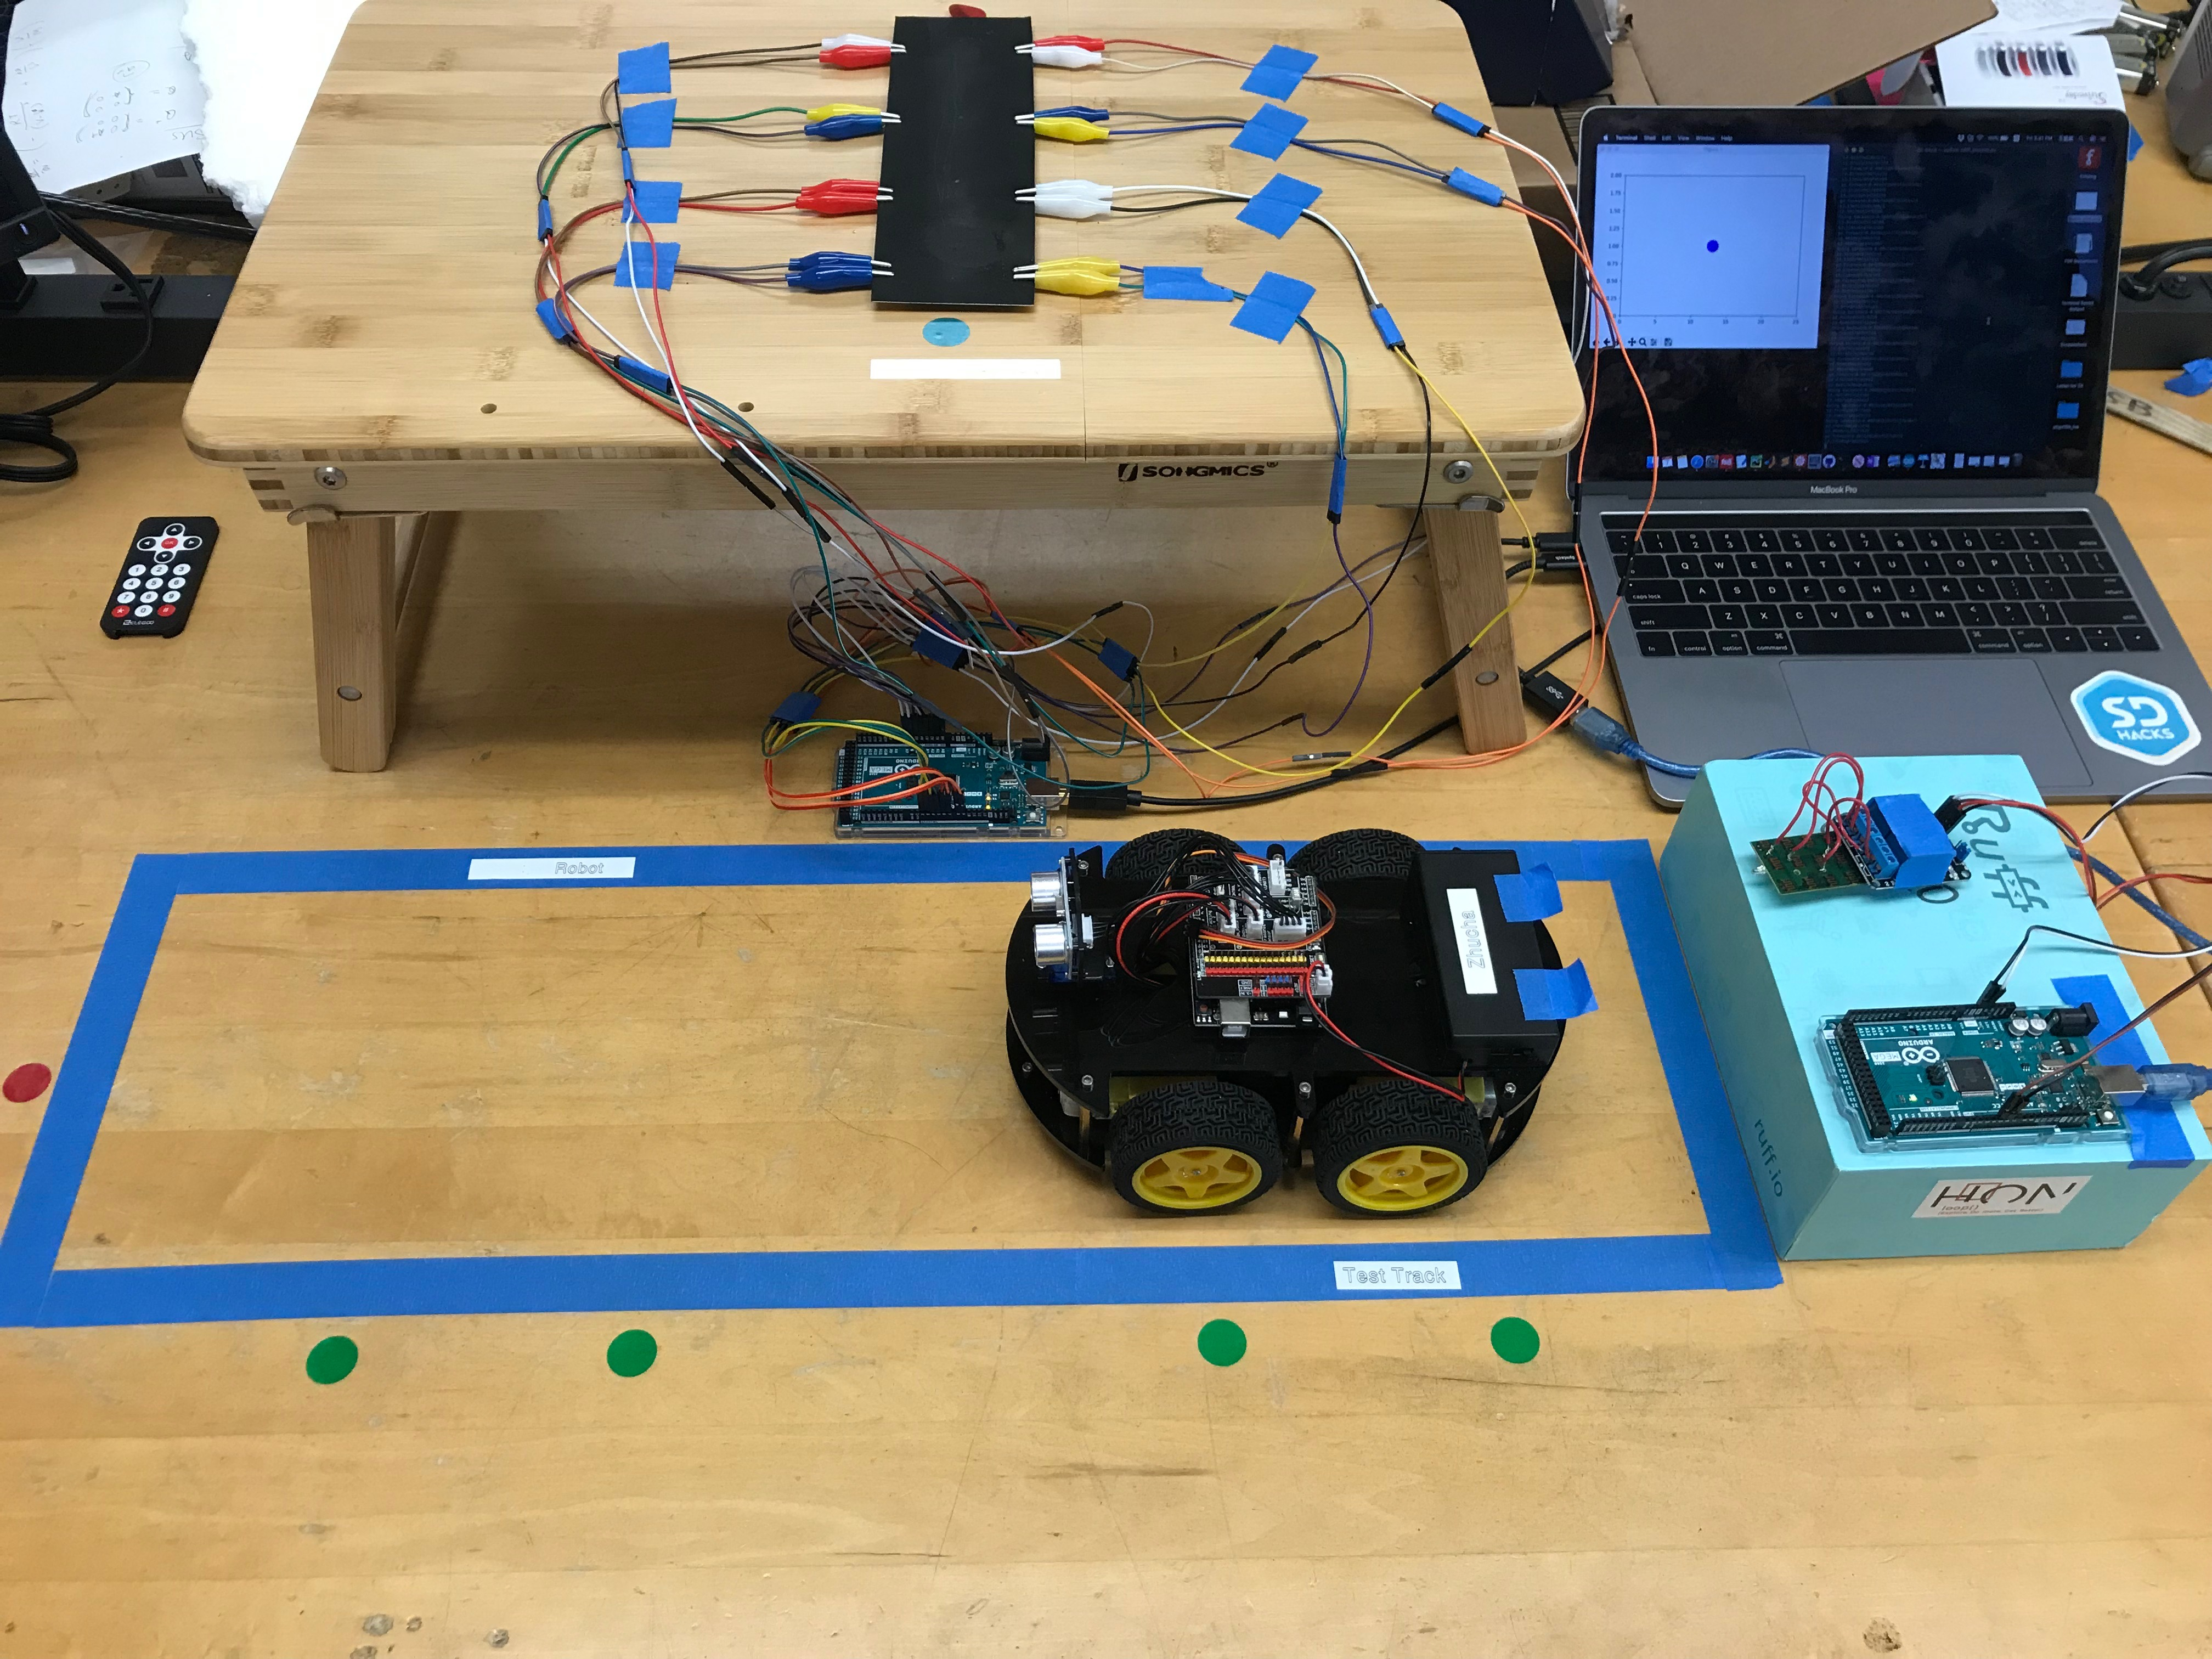
\includegraphics[width=0.4\textwidth]{./figure/setup}     
       \caption{Setup of ROV and touching pad }
    \label{fig::setup}
\end{figure}

\section{Touching Pad}
The goal of the touching pad is that it can be manufactured by shrinking the real size of the actual terrain where the ROV operates. Then, any touching on the touching pad will correspond to a real coordinate in the actual terrain. Therefore, the command applied on the touching pad will correspond to a command of the ROV in the real field. In this section, we are going to introduce the method we constructed the touching pad and the mechanism we use to sense the touch.

\subsection{Electric sensing principle}
Our sensing principle is based on the a carbon-coated plastic board which changes its resistance distribution when the mechanical deformation happens on the board. We also call this method Dynamic Pressure Sensing since as we put our finger on the board, the contact pressure creates the local deformation on the board. This deformation leads to a change in the resistance distribution of the board. 

In Fig. \ref{fig::pressure}, DC current is used to describe the shift of voltage created by the pressing of the finger. When no pressure is applied on the material, the voltage stays constant, which we called baseline. As we may observe, the press of the finger cause an increase of the voltage. When we release the finger, the voltage drops back to the the line which is close to the initial voltage. However, one thing deserved notice is that the voltage does not drop back to the baseline exactly. This phenomenon introduces 3 \% error in this test but we did not consider its effect in our setup of the touching pad. We will discuss the issue in details in the section for future improvement.

\begin{figure}[h]
\centering
    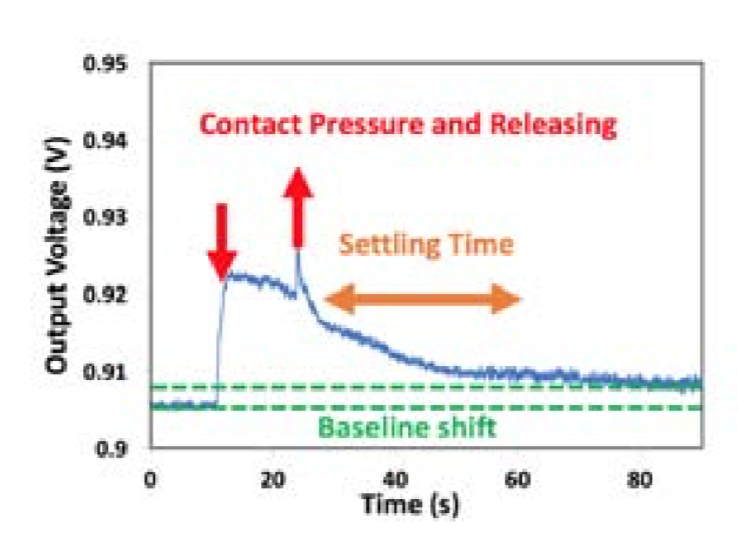
\includegraphics[width=0.45\textwidth]{./figure/pressure}     
       \caption{Voltage reading from a sensing channel fed with fixed DC current upon pressure. The green line (baseline) represent the voltage when no pressure is applied on the board, while the blue line describe the voltage shift caused by the pressing and releasing of the finger. \citep{isoft} }
    \label{fig::pressure}
\end{figure}

In addition, we also tried to implement another popular sensing mechanism based on electric shunting \cite{shunt}, which is implemented by Zhang \cite{electrick}. This mechanism is wildly utilized in Electric Field (EF) sensing systems \cite{ef}. However, this principle requires generating high frequency (200Khz) AC current and higher standard for noise reduction. The wave generator we used, Arduino Mega 2560 \citep{arduino}, cannot generate clean enough signal and the effect of electric shunting cannot be detected from the measurement. Hence, we choose to use the dynamic pressure sensing as our sensing principle.
\subsection{Touching pad setup}
The touching pad is constructed by spraying a conductive carbon paint made by MG Chemicals \citep{carbon} on the surface of a plastic board (25cm $\times$ 6cm). Eight electrodes are placed on the peripheral of the board with separation 6cm and each electrode is consist of 2 alligator clips with one of them applying the voltage and the other measures the voltage. Each 
\begin{figure}[h]
\centering
    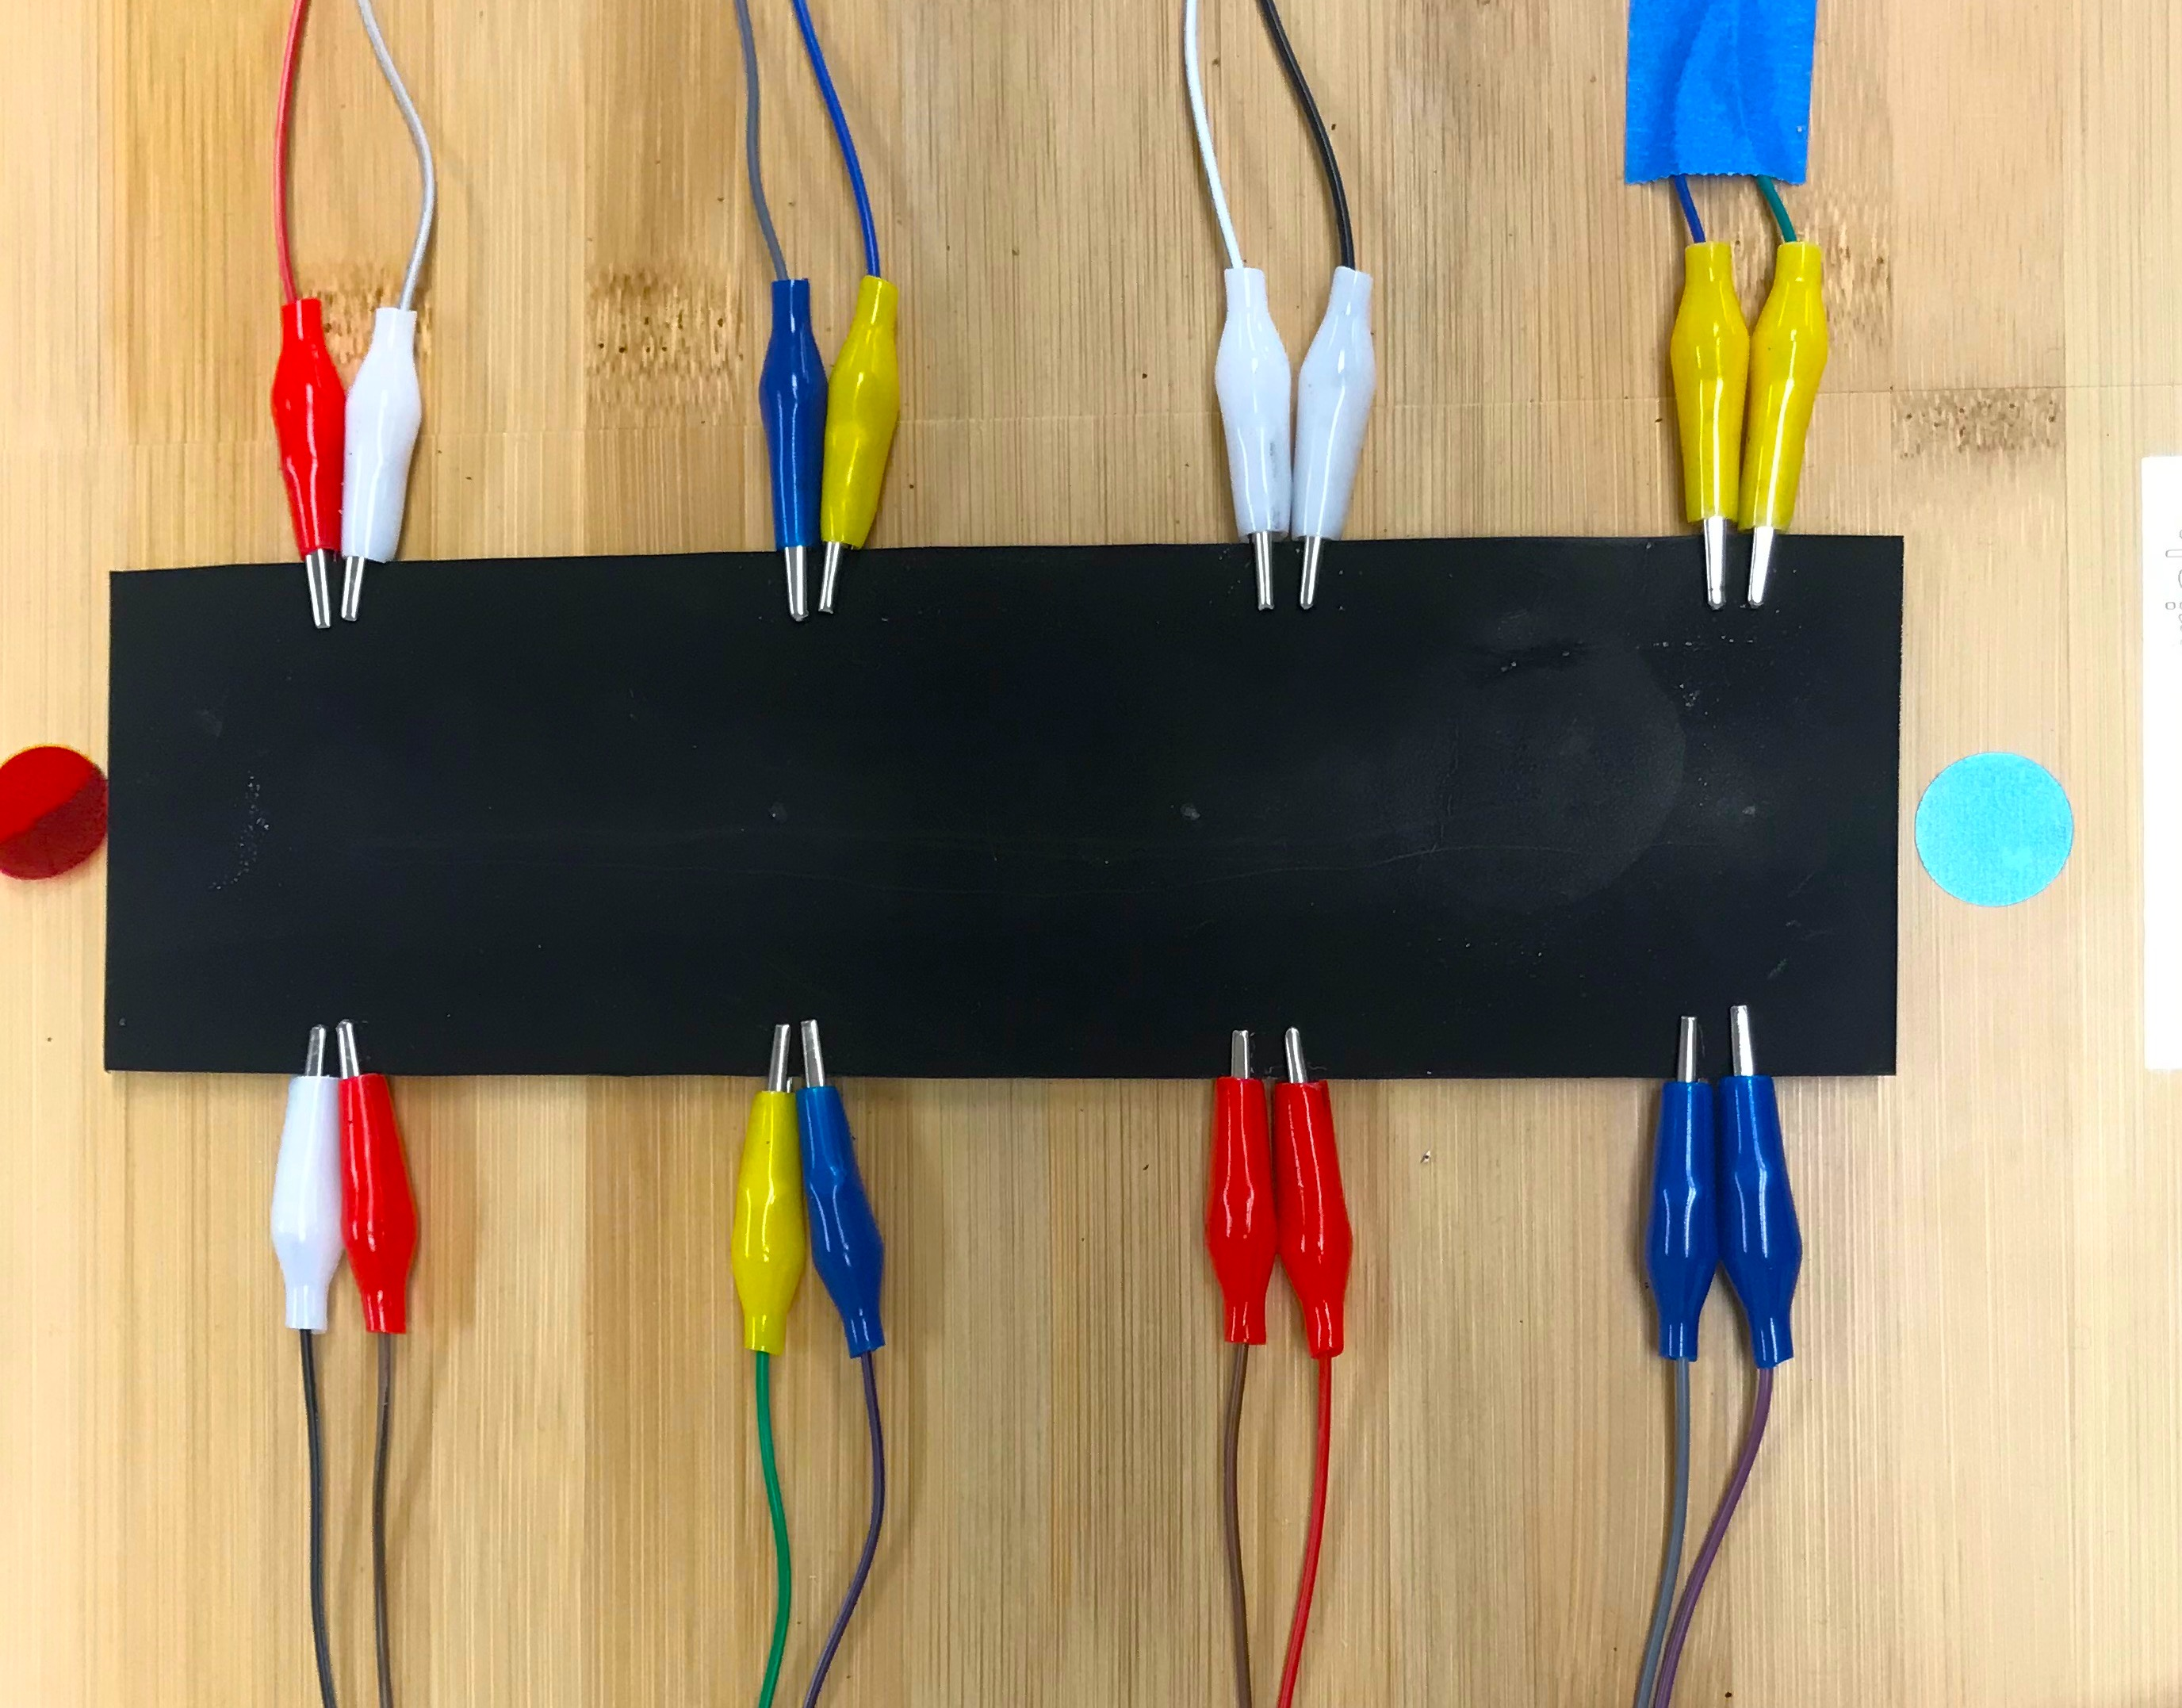
\includegraphics[width=0.45\textwidth]{./figure/pad}     
       \caption{. \citep{isoft} }
    \label{fig::pad}
\end{figure}
\subsection{Measuring procedures}
\subsection{Implementation}

\section{Visualization and Finger Localization}
\subsection{Voltage color-map}
\subsection{Machine learning for finger localization}

\section{Remotely Operated Robot (ROV)}
\subsection{Modules}
\subsection{Control method}
\subsection{Communication with the touching pad}

\section{Future Improvement}
\subsection{•}

\nocite{*}
\bibliography{rov}% Produces the bibliography via BibTeX.

\end{document}



